% !TEX TS-program = pdflatexmk
\documentclass[12pt]{amsart}

%\usepackage[parfill]{parskip}    % Activate to begin paragraphs with an empty line rather than an indent

\usepackage[margin=1in]{geometry}

\usepackage{amsmath,amssymb,amsthm,latexsym,graphicx}
\usepackage[normalem]{ulem}
\usepackage{setspace} %used for doublespacing, etc.
\usepackage{hyperref}
\usepackage{cancel}
\usepackage[dvipsnames,usenames]{color}
\usepackage[all]{xy}
\DeclareGraphicsRule{.tif}{png}{.png}{`convert #1 `dirname #1`/`basename #1 .tif`.png}

%Some useful environments.
\newtheorem{theorem}{Theorem}
\newtheorem{corollary}[theorem]{Corollary}
\newtheorem{conjecture}[theorem]{Conjecture}
\newtheorem{lemma}[theorem]{Lemma}
\newtheorem{proposition}[theorem]{Proposition}
\newtheorem{definition}[theorem]{Definition}
\newtheorem{example}[theorem]{Example}
\newtheorem{axiom}{Axiom}
\theoremstyle{remark}
\newtheorem{remark}{Remark}
\newtheorem*{exercise}{Exercise}%[section]

%Some useful shortcuts for our favorite fields
\newcommand{\RR}{{\mathbb R}}
\newcommand{\NN}{{\mathbb N}}
\newcommand{\ZZ}{{\mathbb Z}}
\newcommand{\QQ}{{\mathbb Q}}
\newcommand{\CC}{{\mathbb C}}

%Some useful shortcuts for formatting lists
\newcommand{\bc}{\begin{center}}
\newcommand{\ec}{\end{center}}
\newcommand{\be}{\begin{enumerate}}
\newcommand{\ee}{\end{enumerate}}
\newcommand{\bi}{\begin{itemize}}
\newcommand{\ei}{\end{itemize}}

%Some useful shortcuts for formatting mathematical symbols
\newcommand{\ol}[1]{\overline{#1}}
\newcommand{\oimp}[1]{\overset{#1}{\Longleftrightarrow}} %labeled iff symbol
\newcommand{\bv}[1]{\ensuremath{ \vec{\mathbf{#1}}} } %makes a vector.
\newcommand{\mc}[1]{\ensuremath{\mathcal{#1}}} %put something in caligraphic font
\newcommand{\mpg}[1]{\marginpar{ #1}} %to put comments in margins
\newcommand{\bsl}[1]{\texttt{\symbol{92}{\em #1}}} %for backslashes.
\newcommand{\normale}{\trianglelefteq}
\newcommand{\normal}{\triangleleft}

%Commenting tools
\usepackage{soul}
\definecolor{highlight}{rgb}{1,0.6,0.6}
\sethlcolor{highlight}
\newcommand{\hlm}[1]{\colorbox{highlight}{$\displaystyle #1$}}
\newtheoremstyle{mycomment}{\topsep}{-0in}{\small \itshape \sffamily}{}{\small \itshape\sffamily}{:}{.5em}{}
\theoremstyle{mycomment}
\newtheorem*{acomment}{\color{BrickRed}{Comment}}
\newcommand{\com}[1]{{\color{OliveGreen}\begin{acomment}{#1} %#2 \color{black} 
\end{acomment}\noindent}}
%\newcommand{\com}[1]{{\color{BrickRed}{\\ Comment:}\color{OliveGreen}{#1} \\}}
\newcommand{\red}[1]{{\color{BrickRed} #1}}
\newcommand{\blue}[1]{{\color{MidnightBlue}#1}}
\newcommand{\green}[1]{{\color{OliveGreen}#1}}
\newcommand{\mwrong}[2]{\red{\cancel{#1}}\green{#2}}
\newcommand{\wrong}[2]{\red{\sout{#1}}\green{#2}}
\definecolor{OliveGreen}{rgb}{.3,.5,.2}
\definecolor{MidnightBlue}{rgb}{.3,.4,.6}

\title{Assignment \#2 Due 9/14/22}

\author{Coordinator: Coordinator's Name}
\begin{document}
\maketitle
%\setstretch{2.5} %Use for 2.5 spacing
\doublespacing %Use for double spacing

% \begin{exercise}[1.7.1 --- Author Name] A sample exercise statement. Be sure to put the name of the person who wrote up this problem's solution in the indicated spot, as well as the name of this week's coordinator. Feel free to modify the \bsl{author} field and omit them for your personal assignment.
% \begin{proof} A sample solution \hl{statement}. 
% \end{proof}
% \com{What's up with that?}
% \end{exercise}

%------------------------------------------------------------
\section*{\textbf{Section 1.6}}
%------------------------------------------------------------


\begin{exercise}[\textbf{1.6.2} --- Stefano Fochesatto]If $\varphi: G \to H$ is an isomorphism, prove that $|\varphi(x)| = |x|$ for all $x \in G$. Deduce that any two 
  isomorphic groups have the same number of elements of order $n$ for each $n\in \ZZ^+$. Is the result true if $\varphi$ is only assumed to be a homomorphism.  
  \begin{proof} Let $\varphi: G \to H$ be an isomorphism and suppose $x \in G$ such that $|x| = \alpha$. By properties of homomorphisms,
    \begin{equation*}
        \varphi(x)^\alpha = \varphi(x^\alpha) = \varphi(e) = e. 
    \end{equation*}
    Suppose there is a $\beta < \alpha$ such that $\varphi(x)^{\beta} = e$. By properties of homomorphisms it would follow that, $x^\beta = e$ which is clearly a contradiction.\\
    Since $\varphi$ is a bijection, by the previous result if there are $m$ elements in $G$ of order $n$ there must be $m$ elements in $H$ of order $n$. This conclusion does not hold 
    if $\varphi$ is only a homomorphism, consider $\varphi: \ZZ_4 \to \ZZ_3$ such that $\varphi(x) = x \mod 3$. There are two elements in $\ZZ_4$ of order 4, and none in $\ZZ_3$ .
  \end{proof}
\end{exercise}
\vspace{.15in}



\begin{exercise}[\textbf{1.6.5} --- Oleksandr Bobrovnikov]
  Prove that the additive groups $\RR$ and $\QQ$ are not isomorphic.
  \begin{proof}[Solution:]
    Suppose this two groups are isomorphic. Then there exists isomorphism $\varphi:\RR\to\QQ$, which is a bijection. But such bijection cannot exist as $\RR$ is uncountable set, and $\QQ$ is countable set. Thus this two groups are not isomorphic.
  \end{proof}
\end{exercise}
\vspace{.15in}



\begin{exercise}[\textbf{1.6.6} --- Glen Woodworth] Prove that the additive groups $\ZZ$ and $\QQ$ are not isomorphic. 
  \begin{proof}
  By way of contradiction, suppose that $\ZZ\cong\QQ$. There exists isomorphism $f:\QQ\rightarrow\ZZ$. Then there exists $q\in\ZZ$ such that $f(q)=1$. Observe,
  \[1=f(q)=f\left(\frac{q}{2}+\frac{q}{2}\right)=f\left(\frac{q}{2}\right)+f\left(\frac{q}{2}\right).\]
  This is a contradiction because there does not exist an integer $n$ such that $n+n=1$. Hence $\ZZ$ and $\QQ$ are not isomorphic.
  \end{proof} 
  \end{exercise}
\vspace{.15in}



\begin{exercise}[\textbf{1.6.14} --- Oleksandr Bobrovnikov]
  Let $G$ and $H$ be groups and let $\varphi:G\to H$ be a homomorphism. Define the kernel of $\varphi$ to be $\left\{ g\in G\,\middle\vert\,  \varphi(g)=1_H \right\}$ (so the kernel is the set of elements in $G$ which map to the identity of $H$, i.e., is the fiber over the identity of $H$). Prove that the kernel of $\varphi$ is a subgroup (cf. Exercise 26 of Section 1 ) of $G$. Prove that $\varphi$ is injective if and only if the
  kernel of $\varphi$ is the identity subgroup of $G$.
  \begin{proof}[Solution:]
    To prove that $\ker \varphi$ is a subgroup in $G$ we must show that for every $x,y\in\ker \varphi$, $xy\in\ker\varphi$, and $x^{-1}\in\ker \varphi$. As $x,y\in\ker\varphi$, $\varphi(x)=\varphi(y)=1$.
    Then $\varphi(xy)=\varphi(x)\varphi(y)=1\cdot 1=1$, as $\varphi$ is a homomorphism. Now as
    $1=\varphi(1)=\varphi(xx^{-1})=\varphi(x)\varphi(x^{-1})=\varphi(x^{-1})$, we deduce that $x^{-1}\in\ker\varphi$.

    Now suppose $\ker \varphi =1$ and $\varphi(x)=\varphi(y)$. As $\varphi$ is a homomorphism, $1=\varphi(x)\varphi(y)^{-1}=\varphi(x)\varphi(y^{-1})=\varphi(xy^{-1})$. And thus $xy^{-1}=1$. So $y^{-1}$ is inverse for $x$, and then $x=y$. So $\varphi$ is injective.

    Suppose $\varphi$ is injective. This implies that if $\varphi(x)=\varphi(y)$, then $x=y$. Let $x\in\ker\varphi$, i.e. $\varphi(x)=1$. We know that as $\varphi$ is a homomorphism, $\varphi(1)=1$. Then from injectivity we obtain that $x=1$. Thus $\ker \varphi =\left\{ 1 \right\}$.
  \end{proof}
\end{exercise}
\vspace{.15in}



\begin{exercise}[\textbf{1.6.15} --- Robert Babac]  
  Define a map $\pi:\mathbb R^2\to\mathbb R$ by $\pi((x,y))=x$. Prove that $\pi$ is a homomorphism and find the kernel of $\pi$ (cf. Exercise 14). 
  \begin{proof}[Solution:]
  Let $(x_1,y_1),(x_2,y_2)\in\mathbb R^2$ where $\pi((x_1,y_1))=x_1$ and $\pi((x_2,y_2))=x_2$. Then $\pi((x_1,y_1)(x_2,y_2))=\pi((x_1x_2,y_1y_2))=x_1x_2=\pi((x_1,y_1))\pi((x_2,y_2))$. Thus, $\pi$ is a homomorphism. $\ker\pi=\{(x,y)\in\mathbb R^2|\pi((0,y))=0\}$
  \end{proof}
  \end{exercise}
\vspace{.15in}



\begin{exercise}[\textbf{1.6.17} --- Glen Woodworth] Let $G$ be any group. Prove that the map from $G$ to itself defined by $g\mapsto g^{-1}$ is a homomorphism if and only if $G$ is abelian.
    \begin{proof} Suppose $f:G\rightarrow G$ such that $f(g)=g^{-1}$. Let $g_1,g_2\in G$. Observe,
    \begin{align*}
    f\text{ is a homomorphism}&\iff f(g_1g_2)=f(g_1)f(g_2)\\
    &\iff (g_1g_2)^{-1}=(g_1)^{-1}(g_2)^{-1}\\
    &\iff (g_1g_2)(g_1g_2)^{-1}=(g_1g_2)(g_1)^{-1}(g_2)^{-1}\\
    &\iff 1_G=(g_1g_2)(g_1)^{-1}(g_2)^{-1}\\
    &\iff g_2g_1=(g_1g_2)(g_1)^{-1}(g_2)^{-1}g_2g_1\\
    &\iff g_2g_1=g_1g_2\\
    &\iff G\text{ is abelian.}
    \end{align*}
    \end{proof} 
\end{exercise}
\vspace{.15in}



\begin{exercise}[\textbf{1.6.18} --- Robert Babac]  
  Let $G$ be any group. Prove that the map from $G$ to itself defined by $g\mapsto g^2$ is a homomorphism if and only if $G$ is abelian.
  \begin{proof}[Solution:]
  $(\Rightarrow)$\\
  Suppose the map $\phi$ from $G$ to itself is defined by $g\mapsto g^{2}$ is a homomorphism. Let $g_1,g_2\in G$. Notice that $g_1g_2g_1g_2=\phi(g_1g_2)=\phi(g_1)\phi(g_2)=g_1g_1g_2g_2$. That is, $g_1g_2g_1g_2=g_1g_1g_2g_2$. By multiplying the inverse of $g_1$ to the left and the inverse of $g_2$ to the right to both sides of the equation, we get $g_1^{-1}g_1g_2g_1g_2g_2^{-1}=g_1^{-1}g_1g_1g_2g_2g_2^{-1}\implies g_2g_1=g_1g_2$. Therefore, $G$ is abelian.\\
  $(\Leftarrow)$\\
  Suppose $G$ is abelian. Let $g_1,g_2\in G$. Then, $\phi(g_1g_2)=(g_1g_2)^{2}=(g_1g_2)(g_1g_2)=(g_1g_1)(g_2g_2)=g_1^{2}g_2^{2}=\phi(g_1)\phi(g_2)$. Therefore, $\phi$ is a homomorphism.\\
  Thus, the map from $G$ to itself defined by $g\mapsto g^{2}$ is a homomorphism if and only if $G$ is abelian.
  \end{proof}
  \end{exercise}
\vspace{.15in}



\begin{exercise}[\textbf{1.6.19} --- Glen Woodworth] Let $G=\{z\in\CC\vert z^n=1\text{ for some }n\in\ZZ^+\}$. Prove that for any fixed integer $k>1$ the map from $G$ to itself defined by $z\mapsto z^k$ is a surjective homomorphism but is not an isomorphism.
  \begin{proof} Fix $k\in\ZZ$ such that $k>1$. Suppose $f:G\rightarrow G$ where $f(z)=z^k$. We first show that $f$ is well-defined. Let $z_1=z_2$ for some $z_1,z_2\in G$. Then $f(z_1)=z_1^k=z_2^k=f(z_2)$. Thus, $f$ is well-defined. We now show $f$ is a surjection. Let $y\in G$. Then there exists $n\in\ZZ^+$ such that $y^n=1$. Then $nk\in\ZZ^+$. We have $(y^{1/k})^{nk}=y^n=1$, so that $y^{1/k}\in G$. Thus, $f(y^{1/k})=y$, so $f$ is surjective. We now show $f$ is a homomorphism. Note that $G\subset\CC$. Then, since $\CC$ is abelian, $G$ is abelian as well. Let $q,t\in G$. Then there exists $n_1,n_2\in\ZZ^+$ such that $q^{n_1}=t^{n_2}=1$. Since $G$ is abelian, we have 
  \[f(qt)=(qt)^{k}=q^{k}t^k=f(q)f(t).\]
  Thus, $f$ is a homomorphism. To see that $f$ is not an injection, note that when $z\in\CC$, $z^k=1$ has $k>1$ distinct roots, all of which will be in $G$ by definition. Hence, there are $k$ unique elements in $G$ such that $f(z)=z^k$, so $f$ is not an injection.
  \end{proof} 
\end{exercise}
  



%------------------------------------------------------------
\section*{\textbf{Section 1.7}}
%------------------------------------------------------------



\begin{exercise}[\textbf{1.7.3} --- Oleksandr Bobrovnikov]
  Show that the additive group $\RR$ acts on the $x,y$ plane $\RR\times\RR$ by $r\cdot(x,y)= (x+ry,y)$.
  \begin{proof}[Solution:]
    We must show that for every $r,s\in\RR$ and for every $(x,y)\in\RR^2$ holds $s(r((x,y)))=(s+r)(x,y)$, and that
    $0(x,y)=(x,y)$. Indeed,
    \begin{equation}
      s(r(x,y))=s(x+ry,y)=(x+ry+sy,y)=(x+(r+s)y,y)=(r+s)(x,y);
    \end{equation}
    \begin{equation}
      0(x,y)=(x+0y,y)=(x,y).
    \end{equation}
  \end{proof}
\end{exercise}
\vspace{.15in}



\begin{exercise}[\textbf{1.7.4} --- Stefano Fochesatto] Let $G$ be a group acting on a set $A$ and fix some $a \in A$. 
  Show that the following sets are subgroups of $G$. 
  \begin{enumerate}
    \item[a.] The kernel of the action, 
    \begin{proof} Let $g, h$ be in the kernel of the action of $G$ and $x \in A$.  Clearly the kernel of the action of $G$ is non empty since it contains the identity. 
      Consider $gh$ acting on $x \in A$, since 
      $g,h$ are in the kernel we get the following, 
      \begin{equation*}
        (gh)\cdot x = (g\cdot (h\cdot x)) = (g \cdot x) = x.
      \end{equation*} 
      Thus $gh$ is in the kernel of the action of $G$. Therefore the group is closed with respect to function composition. Note that,
      \begin{equation*}
        g^{-1}\cdot (x) = g^{-1}\cdot (g \cdot (x)) = (g^{-1}g) \cdot (x) = 1 \cdot x = x.
      \end{equation*}
      Therefore $g^{-1}$ is in the kernel of the action of $G$, therefore the group is closed with respect to inverses. Thus the 
      kernel of the action of $G$ is a subgroup of $G$. 
    \end{proof}
    \vspace{.15in}



    \item[b.] $ Stab_G(a) = \{g \in G | ga = a \}$. \\
    \begin{proof}Let $g, h \in Stab_G(a)$. Clearly $Stab_G(a)$ is non empty since it must contain the identity. Consider $gh$ acting on $a$, since 
      $g,h$ are in the stabilizer group of $a$ in $G$ we get, 
      \begin{equation*}
        (gh)\cdot a = (g\cdot (h\cdot a)) = (g \cdot a) = a.
      \end{equation*} 
      Thus $gh \in Stab_G(a)$ . Therefore the group is closed with respect to function composition. Note that,
      \begin{equation*}
        g^{-1}\cdot (a) = g^{-1}\cdot (g \cdot (a)) = (g^{-1}g) \cdot (a) = 1 \cdot a = a.
      \end{equation*}
      Therefore $g^{-1}\in Stab_G(a)$, therefore the group is closed with respect to inverses. Thus $Stab_G(a) \subseteq G$. 
      
    \end{proof}
  \end{enumerate}
\end{exercise}
\vspace{.15in}



\begin{exercise}[\textbf{1.7.6} --- Oleksandr Bobrovnikov]
  Prove that a group $G$ acts faithfully on a set $A$ if and only if the kernel of the action is the set consisting only of the identity.
  \begin{proof}[Solution:]
    An action is faithful if the only element $g\in G$ such that for every $a\in A$, $ga=a$ is identity element.
    Kernel is the set of the elements of $G$ which fix all the elements of $A$. So action is faithful iff kernel consists only of the identity element.
  \end{proof}
\end{exercise}
\vspace{.15in}



\begin{exercise}[\textbf{1.7.15} --- Stefano Fochesatto] Let $G$ be any group and let $A = G$. Show that the maps defined by $g \cdot a = ag^{-1}$ for all $g, a \in G$
  do satisfy the axioms of a left group action of $G$ on itself.\\
  \begin{proof} Let $G$ be any group and let $A = G$. Suppose the maps defined by $g \cdot a = ag^{-1}$ for all $g, a \in G$. Consider,
    \begin{equation*}
      (gh) \cdot a = a(gh)^{-1} = a(h)^{-1}(g)^{-1} = (g\cdot(h \cdot a)). 
    \end{equation*}
    Also note, 
    \begin{equation*}
      1 \cdot a = a (1)^{-1} = a
    \end{equation*}
    Therefore $g \cdot a = ag^{-1}$  defines a group action on itself.  
  \end{proof}
\end{exercise}
\vspace{.15in}



\begin{exercise}[\textbf{1.7.16} --- Robert Babac]  
  Let $G$ be a group and let $A=G$. Show that the map defined by $g\cdot a=gag^{-1}$ for all $g,a\in G$ \textit{do} satisfy the axioms of a (left) group action (this action of $G$ on itself is called conjugation).
  \begin{proof}[Solution:]
  Let $g_1,g_2,a,e\in G$ where $e$ is the identity element of $G$. Then, $g_1\cdot (g_2\cdot a)=g_1\cdot g_2ag_2^{-1}=g_1g_2ag_2^{-1}g_1^{-1}=(g_1g_2)a(g_1g_2)^{-1}=(g_1g_2)\cdot a$, and $e\cdot a=eae^{-1}=a$. Therefore, the map defined by $g\cdot a=gag^{-1}$ for all $g,a\in G$ \textit{do} satisfy the axioms of a (left) group action.
  \end{proof}
  \end{exercise}
  \vspace{.15in}



\begin{exercise}[\textbf{1.7.17} --- Noah Palmer] Let $G$ be a group and let $G$ act on itself by left conjugation, so each $g\in G$ maps $G$ to $G$ by\\
  \begin{center}
  $x\mapsto gxg^{-1}$
  \end{center}
  For fixed $g\in G$, prove that conjugation by $g$ is an isomoprhism from $G$ onto itself (i.e, is an automorphism of $G$). Deduce that $x$ and $gxg^{-1}$ have the same order for all $x\in G$ and that for any subset $A$ of $G$, $|A|=|gag^{-1}|$ (here $gAg^{-1}=\{gag^{-1}\mid a\in A\}$).
  \begin{proof}
  Let $G$ be a group. For some fixed $g\in G$ we prove that the left conjugation by $g$, that is the function given by $\phi_g(a)=gag^{-1}$, is an isomorphism from $G$ to itself. Let $a,b\in G$ and consider that
  $$\phi_g(ab)=gabg^{-1}=ga(g^{-1}g)bg^{-1}=\phi_g(a)\phi_g(b).$$
  Hence, $\phi_g$ is a homomorphism. We now prove it is a bijection by showing that it is both injective and surjective. To show it is injective we show that $\ker(\phi)=\{1_G\}$, assume for the sake of contradiction there exists $x\in G$ such that $\phi_g(x)=1_G$ and $x\neq 1_G$. This implies that $gxg^{-1}=1_G$. Thus, $gx=g$ and so $x=1_G$, a contradiction. Therefore, the kernel of $\phi_g$ is the set $\{1_G\}$. So, $\phi_g$ is an injection. Next to show that $\phi_g$ is surjective, choose $y\in G$. Then $g(g^{-1}yg)g^{-1}=y$, hence $\phi_g$ is surjective, and thus a bijection. Because $\phi_g$ is a bijection and a homomorphism it follows that it is an isomorphism. \\
  To show that $x$ and $gxg^{-1}$ have the same order, assume that $|x|=n$. Then $\phi(x^n)=gx^ng^{-1}=gxg^{-1}g\ldots gxg^{-1}=(gxg^{-1})^n=1_G$. Thus, $|gxg^{-1}|\leq n$. To show that $|gxg^{-1}|=n$, suppose there exists $m<n$ such that $(gxg^{-1})^m=1_G$. This would imply that $\phi(x^m)=1_G$ which is a contradiction since $|x|=n>m$. Hence, $|x|=|gxg^{-1}|$ for all $x\in G$ and so $|A|=|gAg^{-1}|$.
  \end{proof}
  \end{exercise}
\vspace{.15in}



\begin{exercise}[\textbf{1.7.18} --- Noah Palmer] Let $H$ be a group acting on a set $A$. Prove that the relation $\sim$ defined by 
  $$a\sim b\text{   if and only if   } a=hb\text{   for some   }h\in H$$
  is an equivalence relation. (For each $x\in A$ the equivalence class of $x$ under $\sim$ is called the orbit of $x$ under the action of $H$. The orbits under the action of $H$ partition the set $A$).
  \begin{proof}
  Let $H$ be a group acting on some set $A$, we prove that the relation $\sim$ defined by $a\sim b\text{   if and only if   } a=hb\text{   for some   }h\in H$ is an equivalence relation. First, observe that $a\sim a$ since $a=1_Ha$, and so $\sim$ is reflexive. Next, let $a\sim b$, that is $a=hb$ for some $h\in H$. It follows that $h^{-1}a=b$ and so $b\sim a$. Therefore, $\sim$ is symmetric. Finally, let $a\sim b$ and $b\sim c$. Then $a=hb$ and $b=h^\prime c$ for some $h,h^\prime\in H$. Thus, $a=hh^\prime c$ which implies that $a\sim c$. Hence, $\sim$ is transitive. Since $\sim$ is reflexive, symmetric and transitive we conclude that $\sim$ is by definition an equivalence relation. Therefore, the orbits, that is the equivalence class of $x$ under $\sim$, under the action of $H$ partition the set $A$.
  \end{proof}
  \end{exercise}
\vspace{.15in}



\begin{exercise}[\textbf{1.7.19} --- Noah Palmer] Let $H$ be a subgroup of the finite group $G$ and let $H$ act on $G$ by left multiplication. Let $x\in G$ and let $\mathcal{O}$ be the orbit of $x$ under the action of $H$. Prove that the map 
  $$H\to\mathcal{O}\text{  defined by  } h\mapsto hx$$
  is a bijection (hence all orbits have cardinality $|H|$). From this and the preceding exercise deduce Lagrange's Theorem:\\
  \begin{center}
  if $G$ is a finite group and $H$ is a subgroup of $G$ then $|H|$ divides $|G|$.
  \end{center}
  \begin{proof}
  Let $H$ be a subgroup of some finite group $G$ and let $H$ act on $G$ by left multiplication. Let $x\in G$ we prove that the map $\phi: H\to\mathcal{O}$ defined by $h\mapsto hx$ is a bijection. To show that it is surjective choose $y\in \mathcal{O}$. By defintion $y=gx$ for some $g\in H$ and so $\phi(g)=gx=y$. %Unsure
  Thus, $\phi$ is surjective. Next, suppose $\phi(a)=\phi(b)$. It follows that $ax=bx$ and so $axx^{-1}=bxx^{-1}$ which implies that $a=b$. Thus, $\phi$ is injective. Since $\phi$ is both injective and surjective it follows that $\phi$ is a bijection. Thus, for all $\mathcal{O}\in G$ $|\mathcal{O}|=|H|$.\\
  By the preceding exercise the group action given by $\phi$ partitions $G$ into orbits $\mathcal{O}_1,\ldots,\mathcal{O}_n$ for $n\in\mathbb{N}$, and so $|G|=|\mathcal{O}_1|+\ldots+|\mathcal{O}_n|$. But since we just proved that for all $k$, $|\mathcal{O}_k|=|H|$ it follows that $|G|=n|H|$. Therefore, the order of any subgroup $H$ of $G$ divides $|G|$.
  \end{proof}
  \end{exercise}
\vspace{.15in}



\begin{exercise}[\textbf{1.7.20} --- Robert Babac]  
  Show that the group of rigid motions of a tetrahedron is isomorphic to a subgroup (cf. Exercise 26 of Section 1) of $S_4$.
  \begin{proof}[Solution:]
  Let us first find all the possible rigid motions of a tetrahedron that maps to a unique permutation of 4 elements, let's say $\{1,2,3,4\}$. Notice that 1 rigid motion of the tetrahedron consists of fixing 1 vertex and "rotating" the other three vertices (i.e., if we fix vertex a, then for vertex b, c, d, $b\to c$, $c\to d$, and $d\to a$). For example,
  \begin{center}
      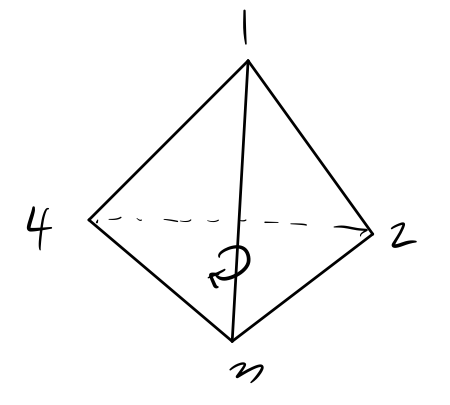
\includegraphics[scale=0.5]{tet 1.jpeg} 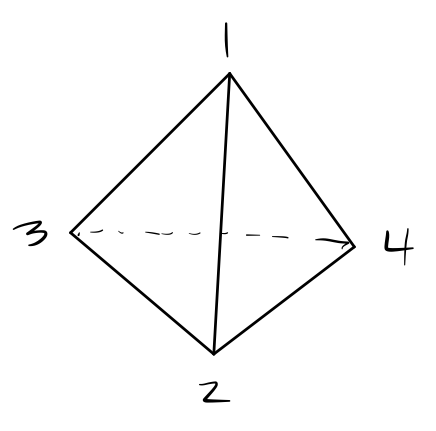
\includegraphics[scale=0.5]{tet 2.jpeg}
  \end{center}
  We can get the trivial rigid motions mapping to the permutations 
  \begin{align*}
      (), (234),(432), (134), (431), (124), (143) (123), \text{ and }(321).
  \end{align*} Note, $()$ is the permutation corresponding to the rigid motion where nothing happens. Notice that for a rigid motion, if we fix vertex a, we cannot also fix vertex b and have only vertices c and d swap places. Thus, we cannot have a rigid motion mapping to the permutations with 1 transposition. That is, we cannot have
  \begin{align*}
      (12),(13),(14),(23),(24),\text{ and }(34).
  \end{align*} By further inspection, we can say any permutation of length 4 will also not be an allowed rigid motion since the decomposition of the permutation consists of the permutation of a rigid motion with 1 transposition. For example, $(1234)=(123)(14)$. Thus, the permutations 
  \begin{align*}
      (1234),(1243),(1324),(1342),(1423),\text{ and }(1432)
  \end{align*} are also not considered rigid motions. We can find the last three rigid motions by below. 
  \begin{center}
      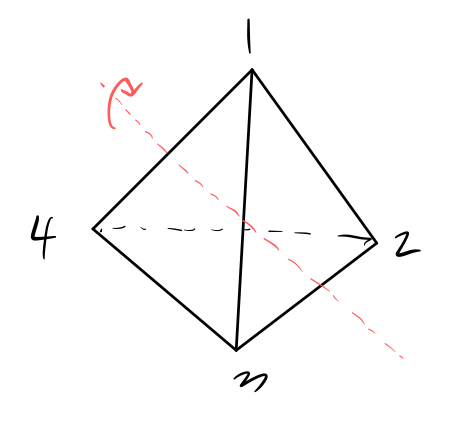
\includegraphics[scale=0.5]{tet rot in 1.jpeg} 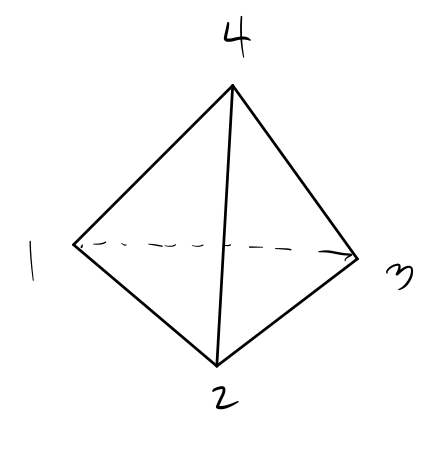
\includegraphics[scale=0.5]{tet rot 1.jpeg}\\
      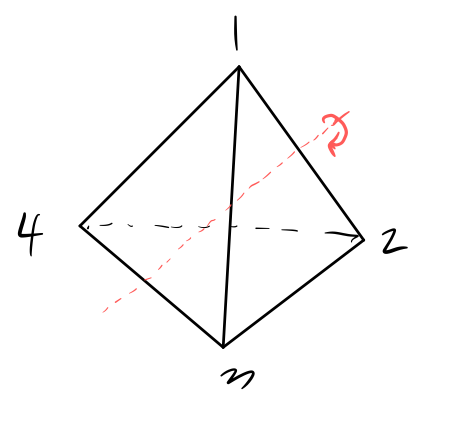
\includegraphics[scale=0.5]{tet rot in 2.jpeg} 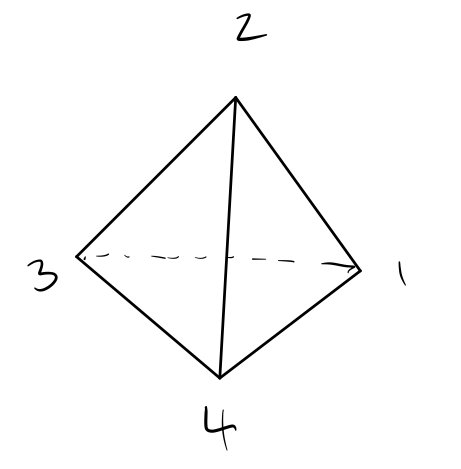
\includegraphics[scale=0.5]{tet rot 2.jpeg}\\
      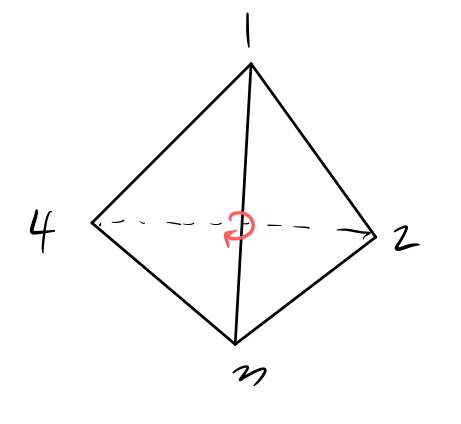
\includegraphics[scale=0.5]{tet rot in 3.jpeg} 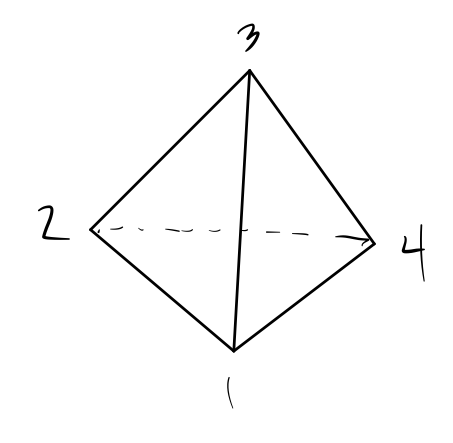
\includegraphics[scale=0.5]{tet rot 3.jpeg}
  \end{center}
  Thus, the last three rigid motions correspond to the permutations, \begin{align*}
      (12)(34),(13)(24),\text{ and }(14)(23). 
  \end{align*}Thus, the group of rigid motions of a tetrahedron is isomorphic to the group of even permutations of $S_4$.
  \end{proof}
  \end{exercise}

  

%------------------------------------------------------------
\section*{\textbf{Section 2.1}}
%------------------------------------------------------------


\begin{exercise}[\textbf{2.1.5} --- Glen Woodworth] Prove that $G$ cannot have a subgroup $H$ with $|H|=n-1$ where $n=|G|>2$.
  \begin{proof} Suppose $n=|G|>2$ and $H\subseteq G$ where $|H|=n-1$. Then $n-1>1$. We have \[n-1\equiv 0\mod n-1.\] Adding 1 to both sides, we have \[n\equiv 1\mod n-1.\] Hence, $|H|=n-1$ does not divide $|G|=n$, so by Lagrange's Theorem, $H$ is not a subgroup of $G$. Since $H$ was chosen arbitrarily from the possible subsets of $G$ with cardinality $n-1$, any subset of $G$ with a cardinality of $n-1$ is not a subgroup of $G$.
  \end{proof}
\end{exercise} 
\vspace{.15in}



\begin{exercise}[\textbf{2.1.6} --- Oleksandr Bobrovnikov]
  \def\abs#1{\left\lvert#1\right\lvert}
  \def\scpr#1{\left\langle #1\right\rangle }
  \def\midd{\,\middle\vert\, }
  Let $G$ be an abelian group. Prove that $\left\{ g\in G\,\middle\vert\,  \abs g <\infty \right\}$ is a subgroup of $G$ (called the torsion subgroup of $G$). Give an explicit example where this set is not a subgroup when $G$ is non-abelian.

  \begin{proof}[Solution:]
    Let $H=\left\{ g\in G\,\middle\vert\,  \abs g <\infty \right\}$ We must show that for every $h_1,h_2\in H$, $h_1h_2\in H$.
    Let $h_1,h_2\in H$. Then there exist $m,n\in\ZZ$ such that  $h_1^m=h_2^n=1$. Then, as $h_1$ and $h_2$ commute, $(h_1h_2)^{mn}=h_1^{mn}h_2^{mn}=1^n\cdot 1^m=1$.
    Inverse element for $h_1$ is $h_1^{m-1}$. Thus torsion subgroup is closed under multiplication and inverses, and is indeed a subgroup of $G$.

    Consider a group $D_{2\cdot\infty}=\scpr{r,s\midd s^2=1,~sr=s^{-1}s}$. Then $\abs s=2$ and $\abs{sr}=2$ as $(sr)^2=srsr=r^{-1}ssr=1$, But $s\cdot sr =r$, and $\abs r=+\infty$. Thus torsion set contains elements $s$ and $sr$, but is not closed under multiplication, as their product has infinite order. So it is not a subgroup.
  \end{proof}
\end{exercise}
\vspace{.15in}



\begin{exercise}[\textbf{2.1.8} --- Stefano Fochesatto] Let $H$ and $K$ be subgroups of $G$. Prove that 
  $H \cup K$ is a subgroup if and only if either $H \subseteq K$ or $K \subseteq H$.
    \begin{proof} Let $H$ and $K$ be subgroups of $G$. Suppose that $H \cup K$ is a subgroup and without loss of generality let $H \not\subseteq K$. 
      Therefore there exists some $h \in H$ such that $h \not\in K$.
      Consider $k \in K$ and note that $hk \in H \cup K$ and since $h \not\in K$, $hk \not\in K$ and therefore it follows that 
      $hk \in H$. Since $H$ is a subgroup $(h^{-1}h)k = k \in H$ and therefore $K \subseteq H$.\\
      For the reverse statement suppose without loss of generality that $K \subseteq H$. Therefore $H\cup K = H$, which is by definition a subgroup. 
    \end{proof}
\end{exercise}
\vspace{.15in}








%------------------------------------------------------------
\section*{\textbf{Section 2.2}}
%------------------------------------------------------------


\begin{exercise}[\textbf{2.2.6} --- Glen Woodworth] Let $H$ be a subgroup of the group $G$. 
  \begin{enumerate}
  \item Show that $H\le N_G(H)$. Give an example to show that this is not necessarily true if $H$ is not a subgroup.
  \item Show that $H\le C_G(H)$ if and only if $H$ is abelian. 
  \end{enumerate}
  \begin{proof}
  (a) Since $H\le G$, $H\ne\emptyset$. Suppose $h_1\in H$. For all $h\in H$, we have $hh_1h^{-1}\in H$ because $H$ must be closed under the binary operation of $G$. Hence, $H\subseteq N_G(H)$, but since $H\le G$, $H\le  N_G(H)$. As an example, suppose $G=S_4$ and $H=\{1,(12)\}$. Then $(12)$ has no inverse in $H$, so $H$ is not a subgroup of $C_G(H)$.\\
  (b) First, note that since $H\le G$, and $C_G(H)\le G$, we have \[H\subseteq C_G(H)\iff H\le C_G(H).\] Now, observe
  \begin{align*}
  H\le C_G(H)&\iff H\subseteq C_G(H)\\
  &\iff  \forall h_1,h_2\in H, h_2h_1h_2^{-1}=h_1\\
  &\iff  \forall h_1,h_2\in H, h_2h_1=h_1h_2\\
  &\iff H \text{ is abelian }.
  \end{align*}
  \end{proof} 
  \end{exercise}
\vspace{.15in}



\begin{exercise}[\textbf{2.2.7} --- Noah Palmer] Let $n\in\mathbb{Z}$ with $n\ge 3$. Prove the following:
  \begin{enumerate}
  \item[(a)] $Z(D_{2n})=1$ if $n$ is odd
  \item[(b)] $Z(D_{2n})=\{1,r^k\}$ if $n=2k$
  \end{enumerate}
  \begin{proof}
  \begin{enumerate}
  \item[(a)] Let $n\in\mathbb{Z}$ where $n$ is a odd and $n\ge 3$. Assume for the sake of contradiction that there exists $g\in Z(D_{2n})$ and $g\neq 1$. Thus, $gx=xg$ for all $x\in G$. We know that $g=s^ir^k$ for some $0\leq k<n$ and $i=0$ or $1$. It follows that $s^ir^ks=s^{i+1}r^k$ which implies that $s^{i+1}r^{-k}=s^{i+1}r^k$ and so $r^k=r^{-k}$. Thus, $r^2k=1$. But this is a contradiction since $n$ is odd and we assumed that $k<n$. Hence, there exists no such elements, and so $Z(D_{2n})=1$.

  \item[(b)] Let $n=2k$ for some $k\in\mathbb{Z}$. Observe that $r^kr^k=1$, so $r^k=r^{-k}$. Now, choose $a\in D_{2n}$ and so $a$ can be expressed in the form $a=s^ir^j$ for $j\in\mathbb{Z}$ and $i=0$ or $1$. Then $r^ks^ir^jr^k=s^ir^{j}r^{k-k}=s^ir^j$, and so $r^k\in Z(D_{2n})$. To show that $r^k$ and $1$ are the only elements in $Z(D_{2n})$, assume for the sake of contradiction that there exists $b=s^ir^m$ such that $bx=xb$ for all $x\in D_{2n}$. Thus, $s^{i+1}r^m=s^ir^ms$ for $0\leq m<2k$ and $i=0$ or $1$. If $i=0$ then $r^ms=sr^{-m}=sr^m$ which implies that $r^m=r^{-m}$ implying that $m=k$, and so $b=r^k$. Instead, if $i=1$ then $sr^ms=s^2r^{-m}=r^{-m}=r^m=s^2r^m$, and so again $b=r^k$. In either, case $b$ is equal to $r^k$ which is a contradiction since we assumed that $b$ was a distinct element of $Z(D_{2n})$. Thus, no such element exists and $Z(D_{2n})=\{1,r^k\}$.
  \end{enumerate}
  \end{proof}
  \end{exercise}
\vspace{.15in}



\begin{exercise}[\textbf{2.2.9} --- Noah Palmer] For any subgroup $H$ of $G$ and any nonempty subset $A$ of $G$ define $N_H(A)$ to be the set $\{h\in H\mid hAh^{-1}=A\}$. Show that $N_H(A)=N_G(A)\cap H$ and deduce that $N_H(A)$ is a subgroup of $H$ ( note that $A$ need not be a subset of $H$).
  \begin{proof}
  Let $H$ be some subgroup of $G$ and let $A$ be some nonempty subset of $A$. Choose $a\in N_H(A)$. It follows by definition that $a\in H$ and $a\in G$. Since $a\in G$ and $aAa^{-1}=A$ it follows that $a\in N_G(A)$. Therefore, $a\in N_G(A)\cap H$. Next choose $b\in N_G(A)\cap H$. It follows that $b\in H$ and $bAb^{-1}=A$ and so by definition $b\in N_H(A)$. Thus, $N_H(A)=N_G(A)\cap H$. Since for all $h\in N_H(A)$, $h\in H$ it follows that $N_H(A)\leq H$.
  \end{proof}
  \end{exercise}
\vspace{.15in}

  

\begin{exercise}[\textbf{2.2.10} --- Stefano Fochesatto] Let $H$ be a subgroup of order 2 in $G$. Show that $N_G(H) = C_G(H)$. Deduce that if $N_G(H) = G$ then $H \subseteq Z(G)$.
  \begin{proof} Let $H$ be a subgroup of $G$ and suppose $H = \{1, h\}$. Consider $g \in N_G(H)$, by definition $gHg^{-1} = H$. By properties of 
    group actions we know that $g1g^{-1} = 1$ and since there is only one other element in $H$ we know that $ghg^{-1} = h$. Therefore $g \in C_G(H)$ and $N_G(H) \subseteq C_G(H)$.
    Consider $g \in C_G(H)$. By definition for all $a \in H$, $gag^{-1} = a$ and therefore $gHg^{-1} = H$. It follows that $g\in N_G(H)$, therefore $C_G(H) \subseteq N_G(H)$. 
    Thus $N_G(H) = C_G(H)$.\\
    If $N_G(H) = G$ by what we have shown $C_G(H) = G$. Therefore for all $h \in H$ and $g \in G$, $ghg^{-1} = h$ which by right cancellation implies $gh = hg$. 
    Since $H$ is a subgroup of $G$, $h \in G$ and therefore by definition $H \subseteq Z(G)$. 
  \end{proof}
\end{exercise}
\vspace{.15in}



\begin{exercise}[\textbf{2.2.11} --- Robert Babac]  
  Prove that $Z(G)\le N_G(A)$ for any subset of $A$ of $G$.
  \begin{proof}[Solution:]
  Let $G$ be a group and $A$ be a subset of $G$. Let $z_1,z_2\in Z(G)$. Then, $z_1g=gz_1$ and $z_2g=gz_2$ for all $g\in G$. Observe that $(z_1z_2)g=z_1(z_2g)=z_1(gz_2)=(z_1g)z_2=(gz_1)z_2=g(z_1z_2)$. That is, $Z(G)$ is closed. Notice that $z_1g=gz_1\implies z_1^{-1}z_1gz_1^{-1}=z_1^{-1}gz_1z_1^{-1}\implies gz_1^{-1}=z_1^{-1}g$ for all $g\in G$. Thus, inverses are in $Z(G)$. Therefore, $Z(G)\le G$.
  \end{proof}
  \end{exercise}
  \vspace{.15in}
  \end{document}